\documentclass[aspectratio=169]{beamer}
\usepackage[backend=biber]{biblatex}
\usepackage{graphicx}
\usepackage{appendixnumberbeamer}
\usepackage{xcolor}
\usepackage{tikz}
\usetikzlibrary{trees}	% this is to allow the fork right path

%https://git-r3lab.uni.lu/R3/outreach/templates/presentations/latex
%https://wwwfr.uni.lu/snt/about_us/snt_presentation2

% theme/ directory contains the actual theme, add it to package loading path
\makeatletter\def\input@path{{theme/}}\makeatother

% load the theme :]
\usetheme{snt}
\usefonttheme[onlymath]{serif}

% the default font theme is snt-fira, you may also try one of:
%\usefonttheme{snt-ibmplex} % IBM technical script
%\usefonttheme{snt-roboto} % roboto + source sans
%\usefonttheme{snt-noto} % very unicode-ish fonts
%\usefonttheme{snt-lmodern} % Knuth style
%\usefonttheme{snt-heros} % Helvetica-style

\usepackage{qrcode} % remove if you don't use QR codes
\usetikzlibrary{positioning} %remove this if you don't use tikz [below=of something] syntax

% metadata
\title{Talk Title}
\author{Author Name}
\date{BioCore team meeting, Month $X$\textsuperscript{th}, 2021}

% Put the references list on the page following the reference titlepage
\AtBeginBibliography{\newpage}

% Add citation styles
\DeclareFieldFormat[article, inproceedings]{citetitle}{#1}
\newcommand\citet[1]{%
    \textbf{\textit{\citetitle{#1}}}~{\color{snt purple}(\citeauthor{#1},~\citeyear{#1}~\cite{#1})}%
}
\newcommand{\citea}[1]{%
    {\color{snt purple}%
    \citeauthor{#1}~(\citeyear{#1})~\cite{#1}}%
}
\newcommand{\citep}[1]{%
    {\color{snt purple}%
    (\citeauthor{#1},~\citeyear{#1}~\cite{#1})}%
}

% various visual details
\logo{\useboth} %or just \useunilu or \usesnt, or use \includegraphics{...}
\setsntbackground{iwatermark} % `watermark` is also good, see below
\setbeamertemplate{footer text}[authortitle] % footer line
\setbeamertemplate{caption}{\raggedright\insertcaption\par} % remove `Figure:` in captions

% allow a footnote without any citation number in the slide text
\newcommand\blfootnote[1]{%
  \begingroup
  \renewcommand\thefootnote{}\footnote{#1}%
  \addtocounter{footnote}{-1}%
  \endgroup
}

\newcommand\forward[1]{\textcolor{snt purple}{{\textbf{\textit{#1}}}}}
\newcommand\redalert[1]{\textcolor{snt red}{#1}}

\addbibresource{bib.bib}

\setbeamerfont{bibliography entry author}{size=\tiny, series=\bfseries}
\begin{document}

\snttitlepage{bgdefault} %or brain, or microscope

\begin{frame}{Outline}
\begin{enumerate}
  \item First part
  \item Second part
\end{enumerate}
\end{frame}

\begin{frame}{Outline v2}
    \tableofcontents
\end{frame}

\section{First part}

\begin{frame}
\begin{columns}
  \begin{column}{.4\linewidth}
  \textbf{First column}
  \begin{itemize}
    \item Something
    \item Something else
    \item \only<1>{???}\only<2->{Solution}
    \item Too much
    \item Way too much!
  \end{itemize}
\end{column}
\begin{column}{.2\linewidth}
  \centering
  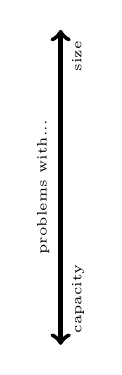
\begin{tikzpicture}[ultra thick]
    \node[anchor=south, font=\tiny, rotate=90] at (0,0) {problems with...};
    \draw[->] (0,0) to node[at end,anchor=north east,rotate=90, font=\tiny] {size} (0,2);
    \draw[->] (0,0) to node[at end,anchor=north west,rotate=90, font=\tiny] {capacity} (0,-2);
  \end{tikzpicture}
\end{column}
\begin{column}{.4\linewidth}
  \textbf{Second column}
  \begin{itemize}
    \item Tiny
    \item Small
    \item \alert<2>{???}
    \item \redalert{Too big}
    \item Plain Bulky
  \end{itemize}
\end{column}
\end{columns}
\end{frame}

\begin{frame}[fragile]{Fragile frames may contain source code}
\begin{verbatim}
\begin{itemize}
  \item Tiny
  \item Small
  \item \alert<2>{???}
  \item Too big
  \item Plain Bulky
\end{itemize}
\end{verbatim}
\end{frame}

\begin{frame}{Blocks}
    \begin{block}{Title}
        \begin{itemize}
            \item[-] This is a block
            \item[-] with
            \item[-] a title
        \end{itemize}
    \end{block}
    
    \begin{block}{}
        This is one without!
    \end{block}
    
\end{frame}


\begin{frame}{Tree Example}
\vspace{1em}
\hspace*{-2.2em}
\begin{tikzpicture}
    \tikzset{
        thick/.style={
            line width=0.8pt
        },
        grow=down, sibling distance=7em,
        every node/.style={
            draw,
            rounded corners=.2em,
            minimum width=20mm,
            text width=18mm,
            align=center,
            font={\scriptsize\bfseries},
            thick,
        },
        sub/.style={
            anchor=west,
            grow=down,
            edge from parent path={(\tikzparentnode.south) |- (\tikzchildnode.west)},
            xshift=1em,
            draw=snt blue
        },
        subnode/.style={
            font={\tiny},
        },
        every child/.style={
            draw=snt blue
        },
        hide/.style={
            opacity=0.2,
        }
    }
    
    \coordinate
        node[style={font=\large\bfseries, text width=60mm, draw=snt blue}]{Anomaly Detection Techniques}
            [edge from parent fork down]
            child {node{Classification Based}
                child[sub, level distance=4em] {node[subnode]{Neural Networks-Based}}
                child[sub, level distance=6em] {node[subnode]{Bayesian Networks-Based}}
                child[sub, level distance=8em] {node[subnode]{Support Vector Machines-Based}}
                child[sub, level distance=9.7em, hide] {node[subnode]{Rule-Based}}
            }
            child {node{Nearest Neighbor-Based}
                child[sub, level distance=4em] {node[subnode]{Using Distance to $k$\textsuperscript{th} Nearest Neighbor}}
                child[sub, level distance=6.5em] {node[subnode]{Using Relative Density}}
            }
            child {node{Clustering-Based}}
            child {node{Statistical}
                child[sub, level distance=4em] {node[subnode]{Parametric}
                    child[sub, dashed, level distance=1.6em, hide] {node[subnode, text width=30mm]{Gaussian Model-Based}}
                    child[sub, dashed, level distance=3.2em] {node[subnode, text width=30mm]{Regression Model-Based}}
                    child[sub, dashed, level distance=5em] {node[subnode, text width=30mm]{Mixture of Parametric\\ Distributions-Based}}
                }
                child[sub, level distance=11em, hide] {node[subnode]{Nonparametric}}
            }
            child[hide] {node{Information Theoretic}}
            child[hide] {node{Spectral}};
\end{tikzpicture}
\end{frame}

\begin{frame}{Tree Example (bis)}
    \centering
    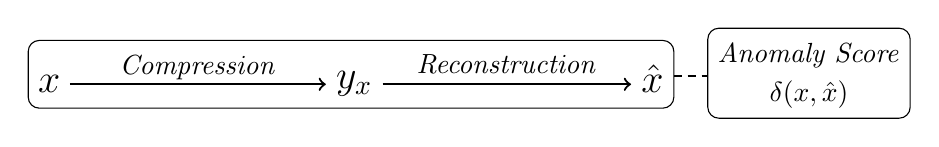
\begin{tikzpicture}
        \tikzset{
            every node/.style={
                align=center,
                text centered,
                anchor=north,
            }
        }
        \node[left] (a) at (0, 0) {\Large $x$};
        \draw[->, thick] (a) -- ++(10em, 0)
            node[above, pos=0.5, yshift=-.2em]{\textit{Compression}}
            node(b)[right]{\Large $y_x$};    
        \draw[->, thick] (b) -- ++(10em, 0)
            node[above, pos=0.5]{\textit{Reconstruction}}
            node(c)[right]{\Large \raisebox{.3em}{$\hat{x}$}};
        \draw[rounded corners] ([yshift=-.2em]a.south west) rectangle ([yshift=.5em]c.north east);

        \node(d)[right] at ([xshift=2em, yshift=.3em]c) {\raisebox{1.5em}{\textit{Anomaly Score}}\\[-1.3em] $\delta(x, \hat{x})$};
        \draw[rounded corners] ([yshift=-.0em]d.south west) rectangle ([yshift=.2em]d.north east);

        \draw[densely dashed] ([yshift=.3em]c.east) -- (d.west);
    \end{tikzpicture}
\end{frame}


\section{Second part}
\subsection{This is a subsection}

\snttitlepage{bghand}
\setsntBlueOnRed %default is RedOnBlue
\setsntbackground{watermark}
\snttitlepage{bghead}

%how to do a single plain white/black frame (good for showing pictures alone)
{\setsntbackground{black}\sntwhitelogostrue
\begin{frame}
\centering
\tikz\node[align=center,text width=.4\paperwidth,fill=white,rounded corners=1em, inner sep=1em]{
\qrcode[height=\linewidth]{https://wwwen.uni.lu/snt}\par
\tiny\tt wwwen.uni.lu/snt
};
\end{frame}
}%the background change doesn't propagate outside of {braces}

\begin{frame}{Main theme features}
\begin{itemize}
\item \texttt{\textbackslash documentclass\{\textbf{beamer}\} \textbackslash usetheme\{\textbf{snt}\}}
\item Loose\&incomplete copy of the Metropolis theme in Luxembourg colors
\item A few pre-imported backgrounds
\item Will be maintained at least for as long as there are \LaTeX\ users in Luxembourg
\end{itemize}

\end{frame}

\begin{frame}{Font check slide}
\begin{itemize}
\item \forward{This} could make ligatures: hifi fifi gaffa
\item this should \underline{not}: \texttt{hifi fifi gaffa}
\item \emph{this should be emphasised}
\item \textbf{bold\emph{emph}} \texttt{mono\textbf{bold\emph{emph}}\emph{emph}}
\item \(\sqrt{\frac{\lambda\gamma}{\sigma\beta}x}\)

\[ \sum_{i\in\{1\dots 10\}} i = 55 \]
\end{itemize}
\end{frame}

\begin{frame}{Citations}
You can cite \citep{Burt1983TheLP} like this
\begin{itemize}
    \item Or like that
    \item \cite{Ma2018InfraredAV}
    \item \citet{Burt1983TheLP}
    \item \citea{Burt1983TheLP}
\end{itemize}
\blfootnote{This is a ``blank"-footnote}
\end{frame}

\begin{frame}[standout]
Stand-out frames!
\vfill

\begin{tikzpicture}[ultra thick]
\node[rectangle, rounded corners, draw] (a) {Clean Ti\emph{k}Z graphics};
\node[rectangle, rounded corners, draw, right=of a] (b) {looks good!};
\draw[->] (a) to (b);
\end{tikzpicture}
\end{frame}

{% scope for footer change
\setbeamertemplate{footer}[textonly]
\setbeamertemplate{footer text}{Customized footer!}

\begin{frame}[fragile]{How to use the original LCSB theme?}
\begin{columns}
\begin{column}{0.6\linewidth}
\begin{enumerate}
\item Obtain the template \\ (a pack of \texttt{sty} files + media)
\begin{itemize}
\item R\textsuperscript{3} GitLab
\item \texttt{howto.lcsb.uni.lu}
\end{itemize}
\item Follow the examples
\begin{itemize}
\item ``normal'' beamer slides should work pretty much as-is
\item have a look at \texttt{slides.tex}
\end{itemize}
\item Suggestions welcome!
\end{enumerate}
\end{column}
\begin{column}{0.4\linewidth}
\tiny
\begin{verbatim}
\begin{frame}{How to use the theme?}
 \begin{enumerate}
  \item Obtain the template \\ (a pack
        of \texttt{sty} files + media)
  \begin{itemize}
   \item R\textsuperscript{3} GitLab
   \item have a look at
         \texttt{slides.tex}
  \end{itemize}
  \item Follow the examples
  \begin{itemize}
   \item ``normal'' beamer slides should
         work pretty much as-is
...
\end{verbatim}
\end{column}
\end{columns}
\end{frame}
}
% \setbeamertemplate{footer}[snt] % reset footer

\begin{frame}[allowframebreaks]
    \printbibliography
\end{frame}


\setsntRedOnBlue
\logo{}
\begin{frame}[standout]
\vskip1ex
Thank you for attention!

\vskip2ex
{\fontsize{66pt}{66pt}\selectfont Questions?}
\vskip2ex
\unilulogoW{height=2cm}\qquad\sntlogoW{height=2cm}
\vspace*{4ex}
\flushright{\scriptsize Base Theme Copyright: \href{https://git-r3lab.uni.lu/R3/outreach/templates/presentations/latex}{\textit{LCSB}}}\\
%\vspace{-.5cm}\flushright{\tiny\normalfont  Modified: \href{https://wwwfr.uni.lu/snt/people/romain_hermary}{Romain HERMARY}}
\end{frame}

\appendix

\begin{frame}{This is...}

\vspace{1cm}
A numbered appendix
    \begin{figure}
        \centering
        \vspace{-.5cm}
        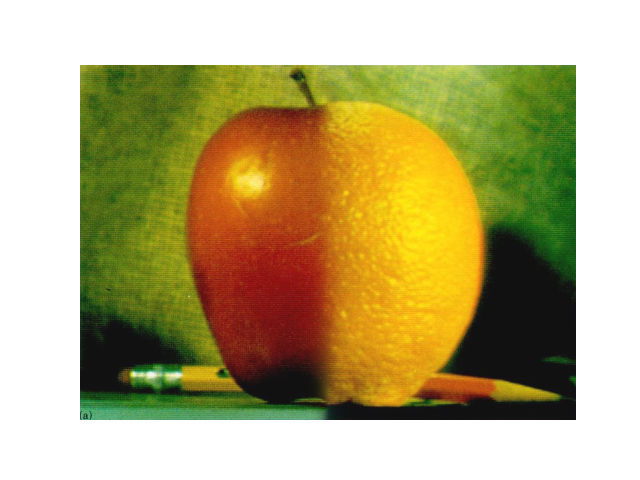
\includegraphics[width=.6\linewidth]{figures/blended.png}
        \vspace{-1cm}\caption{This is a caption}
    \end{figure}
\end{frame}

\end{document}
